%!TEX root = ../bare_jrnl.tex


\section{Introduction}
\label{sec:introduction}

Autonomous mobile robots are being developed to operate in human populated spaces, such as homes and offices~\cite{hawes2016strands}. It is useful for these robots to predict patterns of human activity, so as to learn about those activities~\cite{coppola2016learning,duckworth2016a} or to plan interactions with humans~\cite{2020AAMAS_street}. This paper is concerned with how a robot can correctly estimate how many human activities it has encountered, predict how many will occur in a particular location at a particular time, and then use these to optimize the exploration-exploitation trade-off that occurs during active learning, so as to observe as many human activities as possible during a deployment.

Consider a mobile service robot that works in a large office building. Let us suppose that one of the system designers' aims is for the robot to observe and thereby learn about the various activities performed by humans, and for this learning to have to occur over several days or weeks. To achieve this goal, the robot must learn where and when people are to be found, count the observed activities (perhaps grouped by their categories), and revisit places at times when those activities can be observed in sufficient number. For example, to learn about eating activities the robot would benefit from visiting the canteen at lunchtime, rather than at the start of the day. If such a robot is to be deployed to a variety of buildings, without re-programming of rules by hand, it should autonomously learn the spatio-temporal distribution of these activities and exploit that learning to observe a useful variety and number of activities.

This involves solving two problems. First, the robot must estimate where it can observe the greatest number of human activities at each time of the day. Second, as the robot is learning it should trade-off exploring for new time-place combinations where it might discover a high-level of human activity and re-visiting those time place combinations where it already knows that a wealth of human activity is to be found. This second problem involves solving an exploration-exploitation trade-off. 

\begin{figure}[t!]
	\centering

	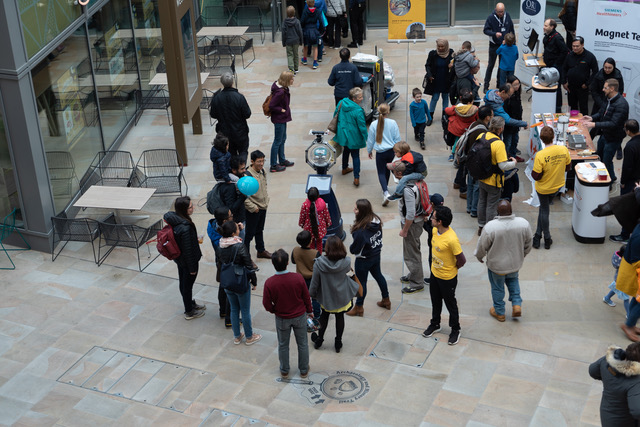
\includegraphics[width=0.5\textwidth]{./figures/robot_in_human_environment.jpeg}
	\caption{Our mobile robot observes people at an event.} 
	\label{fig:robot_in_human_environment}
\end{figure}
This paper presents a Bayesian method to solve both these problems in the case where we treat human activities as count data. %In this approach, there are two sources of uncertainty regarding the number of activities found: human behaviour which has some inherent uncertainty (aleatoric uncertainty) and the robot's uncertainty about what it observed due to it's unreliable sensing (epistemic uncertainty). By representing both types of uncertainty, 
The Bayesian framework models not only the frequency of human activities and the variation in this, but also the robot's uncertainty about the mean rate at which activities occur. Thus, the Bayesian estimator captures both inherent process uncertainty (aleatoric uncertainty) and the robot's additional uncertainty in what it knows about the process (epistemic uncertainty). It can also correct for inherent biases (a tendency to false positives or false negatives in the sensory system). Because of this it has two advantages over a baseline frequentist estimator. First, it will produce more accurate estimates and predictions of human activity levels than a method that does not model classification errors. Second, because it captures epistemic uncertainty it can be used to perform active learning. This active learning problem is fundamentally an exploration-exploitation trade-off. Should the robot visit a place at a time such that it can exploit what it already knows about the likely activity level, or should it explore a place-time combination about which it knows less, but about which it might learn and so lead to a higher rate of activity observation in the long run? This active learning problem is intractable in the strict formulation, since it involves reasoning over a tree of possible knowledge states. Despite this, there are effective, heuristic active-learning rules that are quick to evaluate. %Our main experimental contribution is an active learning scenario in which the robot must learn to efficiently explore a public space so as to learn about human activities quickly.

%The Bayesian framework enables the robot to draw better inferences about the typical level of activity in a particular place time. The Bayesian estimator lends itself to a simple yet effective solution to the exploration-exploitation problem. 
We develop a series of Bayesian estimators. Then we present a method to use these to drive exploration. This uses both a Fourier transform to capture the periodicity of human activities and the epistemic uncertainty in the activity rate as captured by the posterior. Using this estimation, prediction and exploration technique, we then present the results of several long-run deployments of a real robot in a public building. These long-run deployments (15 days per treatment) are used to test whether the different Bayesian estimators, together with the solution to the exploration-exploitation trade-off, result in the robot observing greater numbers of human activities than a baseline frequentist method.

%Our mobile robot has multiple sensors and perception algorithms used to detect humans performing activities. These are inevitably somewhat unreliable. Thus, the raw counts arising from the detectors will be wrong. But, by learning statistical models of the sensor unreliability, the robot can partially correct for these miscounts. In other words, we can teach the robot to count humans more reliably than the raw counts from its detectors. 
This paper builds on our earlier work, which showed how to count reliably from a single unreliable detector or from multiple, unreliable, uncorrelated detectors~\cite{jovan18a}. That work formulated the problem as Bayesian inference for a \textit{partially observable Poisson process} (POPP) and showed an improvement on a baseline model assuming sensor reliability, termed the fully observable Poisson process (FOPP).

This paper makes the following technical contributions. First, we extend the POPP model to create the correlated POPP (C-POPP) model. This supports inference when the robot has multiple detectors with correlated outputs. Second, the observation model used to correct counts in the POPP model is itself constructed from data and so has both epistemic and aleatoric uncertainties. The POPP and C-POPP models only take account of the aleatoric uncertainty in the observation model. We extend the POPP model to include the epistemic uncertainty, resulting in the POPP-Beta model. The third contribution is to combine the benefits of C-POPP and POPP-Beta. This results in the POPP-Dirichlet model, which works for correlated sensors and epistemic uncertainty in the observation model. We demonstrate the inferential properties of POPP and these three extensions in both numerical simulations. The fourth contribution is that we show how these models can be used solve the exploration-exploitation problem by combining Fourier transform that allows us to exploit the periodicity of human activities with an upper bound estimate derived from the posterior. 
Finally, the fifth contribution is an extensive real world evaluation on a long-run robot. We compare the exploration and estimation performance of the FOPP, POPP and POPP-Beta models in a series of three 15-day deployments. Analysis shows that the POPP and POPP-Beta models are able to explore more efficiently, encountering more people than the baseline FOPP model and that they produce superior estimates of the rate of human activities.

%The rest of the paper is organized as follows. We start by describing the  \textit{fully observable Poisson process} as the baseline. We then discuss related works on correcting miscounts. We then review the POPP model and present the three extensions to it. We evaluate all our extensions against both the FOPP and POPP models, doing so on both simulated and real world data. Finally, we present the results of the exploration control study on the robot and summarize our findings.
% 
% We could cut the rest of the paragraph if we're should of space.
% Robot exploration arises from the fact that a mobile robot needs to observe human activities/behaviour in order to adapt to its environment. As the robot has a limit to its operational life, one would therefore like it to optimise the time it takes to build its models. 
% We contrast this with an exploration method based on the FOPP model. We show that the exploration method involving corrections to systematic errors doubles the number of human encounters the robot experiences. 

% We show variations of the exploration methods based on optimistic predictions from the resulting posteriors of the first contribution. 
% BELUM BERES INI
% The second contribution is the variation of exploration methods for a mobile robot based on optimistic predictions from the resulting posteriors of the first contribution. As any mobile robot in human-populated environment needs to learn human behaviour/activity, it must first explore where activities are likely to happened and observe them. One would like the robot to observe a sufficient amount of human activity, so as to learn the specific kinds of activity models. However, as a mobile robot can only be in one place at one time, its observations are spatially restricted. Moreover, the robot has a limit to its operational life. We would therefore like it to optimise the time it takes to build its models. This introduces an exploration-exploitation trade-off problem \cite{wyatt1998exploration, 1413255, AUDIBERT20091876}, i.e. should the robot visit a familiar place, where it will probably observe two activities, or go to a new place, where it might observe many more but might see nothing? 

% is expected to work around and/or with humans, modelling human activities becomes a necessity. In any scenario where a robot learns about human activities, it must first explore where activities are likely to happened and observe them. 
% 
% One would like the robot to observe a sufficient amount of human activity, so as to learn the specific kinds of activity models. However, as a mobile robot can only be in one place at one time, its observations are spatially restricted. Moreover, the robot has a limit to its operational life. We would therefore like it to optimise the time it takes to build its models. This introduces an exploration-exploitation trade-off problem \cite{wyatt1998exploration, 1413255, AUDIBERT20091876}, i.e. should the robot visit a familiar place, where it will probably observe two activities, or go to a new place, where it might observe many more but might see nothing?
% 
% Another important restriction in mobile robotics is that robot sensors are unreliable. Any solution must take into account the unreliability of sensors. We may also require that it do so for when multiple sensors are involved. This means that collected data which are used for learning typically contain systematic errors that lead to bias in the statistical estimates produced by the event detection processes.

% To allow the robot to observe a sufficient amount of human activity, so as to learn the specific kinds of activity models, putting an exploration to places with high number of activities becomes a mandatory action. There are several reasons behind this. First, a mobile robot can only be in one place at one time, so its observations are spatially restricted.   
% 
% The problem of this thesis can be loosely formulated as how to predict where many people are most likely to be and to go and observe them. Specifically, it requires the robot to go to where the aggregate level of human activity is highest. In addition, this thesis chooses to tackle the problem for the case where the robot runs for an extended period of time such days, or even weeks as it builds its models.
% A key challenge is for the robot to be able to recognise and react adequately to dynamic changes that happen in human-centered environments, especially when the changes are the result of human behaviour. The learning process for an autonomous mobile robot to adapt to its environment takes a big portion of its lifetime and it needs to deal with the huge volume of experiences accessible to it as it runs for longer periods of time. One advantage of all these is that these experiences contain potentially useful information that can help the robot to eventually adapt to its environment.

% Taken together, the challenges and benefits faced by an autonomous mobile robot motivate this thesis to create long-term understanding of temporal dynamics of human activities, along with the ability to exploit this understanding for a better adaptation of an autonomous mobile robot. The robot is expected to demonstrate its ability to predict future activities based on its statistical model. It is also expected to be able to detect anomalies as sequences of very low likelihood data.


